% ===========================================================================
%  TikuOS — Processes: Protothreads, Events & Channels
%  Beamer Presentation
% ===========================================================================
\documentclass[aspectratio=169, 10pt]{beamer}

% ---- Theme ----------------------------------------------------------------
\usetheme{Madrid}
\usecolortheme{whale}
\setbeamertemplate{navigation symbols}{}
\setbeamertemplate{footline}{%
  \leavevmode\hbox{%
    \begin{beamercolorbox}[wd=.33\paperwidth,ht=2.5ex,dp=1ex,center]{author in head/foot}%
      \usebeamerfont{author in head/foot}\insertshortauthor
    \end{beamercolorbox}%
    \begin{beamercolorbox}[wd=.34\paperwidth,ht=2.5ex,dp=1ex,center]{title in head/foot}%
      \usebeamerfont{title in head/foot}\insertshorttitle
    \end{beamercolorbox}%
    \begin{beamercolorbox}[wd=.33\paperwidth,ht=2.5ex,dp=1ex,right]{date in head/foot}%
      \usebeamerfont{date in head/foot}\insertshortdate{}\hspace*{2em}%
      \insertframenumber{}/\inserttotalframenumber\hspace*{2ex}
    \end{beamercolorbox}}%
  \vskip0pt%
}

% ---- Packages -------------------------------------------------------------
\usepackage{listings}
\usepackage{graphicx}
\usepackage{hyperref}
\usepackage{booktabs}
\usepackage{multirow}
\usepackage{tikz}
\usetikzlibrary{arrows.meta, positioning, shapes.geometric, calc,
                decorations.pathreplacing, fit}

% ---- Code listing style ---------------------------------------------------
\lstset{
  basicstyle=\ttfamily\scriptsize,
  keywordstyle=\color{blue}\bfseries,
  commentstyle=\color{gray},
  stringstyle=\color{red!70!black},
  showstringspaces=false,
  breaklines=true,
  frame=single,
  rulecolor=\color{black!30},
  backgroundcolor=\color{blue!3},
  tabsize=4,
}
\lstdefinestyle{cstyle}{
  language=C,
  morekeywords={uint8_t,uint16_t,uint32_t,intptr_t,
                tiku_process_t,tiku_event_t,tiku_event_data_t,
                tiku_channel_t,tiku_clock_time_t,
                PT_THREAD,PT_BEGIN,PT_END,PT_YIELD,PT_EXIT,
                PT_EXITED,PT_ENDED,PT_YIELDED,PT_WAITING,
                TIKU_PROCESS,TIKU_PROCESS_WITH_LOCAL,TIKU_PROCESS_TYPED,
                TIKU_PROCESS_THREAD,TIKU_PROCESS_BEGIN,TIKU_PROCESS_END,
                TIKU_PROCESS_YIELD,TIKU_PROCESS_WAIT_EVENT,
                TIKU_PROCESS_WAIT_EVENT_UNTIL,TIKU_PROCESS_EXIT,
                TIKU_AUTOSTART_PROCESSES,TIKU_PROCESS_BROADCAST,
                TIKU_LOCAL,TIKU_THIS,TIKU_CHANNEL_DECLARE,
                TIKU_EVENT_INIT,TIKU_EVENT_EXIT,TIKU_EVENT_TIMER,
                TIKU_EVENT_POLL,TIKU_EVENT_USER,TIKU_EVENT_CONTINUE,
                TIKU_EVENT_FORCE_EXIT,TIKU_EVENT_EXITED,
                TIKU_CLOCK_SECOND,NULL},
}

% ---- Metadata -------------------------------------------------------------
\title[TikuOS Processes]{TikuOS Processes}
\subtitle{Simple. Ubiquitous. Intelligence, Everywhere.}
\author[Ambuj Varshney]{Ambuj Varshney \\ \texttt{ambuj@tiku-os.org}}
\date{\today}

% ===========================================================================
\begin{document}

% ---------------------------------------------------------------------------
\begin{frame}
\titlepage
\end{frame}

% ---------------------------------------------------------------------------
\begin{frame}{Outline}
\tableofcontents
\end{frame}

% ===========================================================================
\section{Why Protothreads?}
% ===========================================================================

\begin{frame}{The Challenge: Concurrency on 2\,KB RAM}
\begin{columns}[T]
\begin{column}{0.48\textwidth}
\textbf{Traditional RTOS threads:}
\begin{itemize}
  \item Each thread needs its own stack
  \item Typical minimum: 128--512 bytes/thread
  \item 4 threads = 512--2048 bytes of stack alone
  \item Impossible on 2\,KB SRAM
\end{itemize}

\vspace{0.5em}
\begin{alertblock}{Stack Overflow}
No MMU means no guard pages.
Stack overflow silently corrupts data.
\end{alertblock}
\end{column}

\begin{column}{0.48\textwidth}
\textbf{Protothreads (TikuOS approach):}
\begin{itemize}
  \item \textbf{Stackless} --- 2 bytes per thread
  \item Cooperative scheduling (no preemption)
  \item Event-driven: sleep until woken
  \item Continuation stored in a single \texttt{lc\_t}
  \item 100+ protothreads on 2\,KB RAM
\end{itemize}

\vspace{0.5em}
\begin{block}{Trade-off}
No local variables across yields ---
use process-local storage instead.
\end{block}
\end{column}
\end{columns}
\end{frame}

% ===========================================================================
\section{Process Data Structures}
% ===========================================================================

\begin{frame}[fragile]{Process Control Block}
\begin{columns}[T]
\begin{column}{0.50\textwidth}
\begin{lstlisting}[style=cstyle,
  title={kernel/process/tiku\_process.h}]
typedef struct tiku_process {
    struct tiku_process *next;
    const char          *name;
    PT_THREAD((*thread)(
        struct pt *,
        tiku_event_t,
        tiku_event_data_t));
    struct pt  pt;
    uint8_t    is_running;
    void      *local;
} tiku_process_t;
\end{lstlisting}
\end{column}

\begin{column}{0.46\textwidth}
\begin{tabular}{@{}lp{4.2cm}@{}}
\toprule
\textbf{Field} & \textbf{Purpose} \\
\midrule
\texttt{next}       & Linked list of active processes \\
\texttt{name}       & Human-readable label \\
\texttt{thread}     & Protothread function pointer \\
\texttt{pt}         & Continuation state (2 bytes) \\
\texttt{is\_running} & Active flag \\
\texttt{local}      & Per-process storage pointer \\
\bottomrule
\end{tabular}

\vspace{0.5em}
\begin{block}{Footprint}
\textasciitilde12 bytes per process on MSP430 (16-bit pointers).
\end{block}
\end{column}
\end{columns}
\end{frame}

% ---------------------------------------------------------------------------
\begin{frame}[fragile]{Event System}
\begin{columns}[T]
\begin{column}{0.48\textwidth}
\textbf{System events:}
\begin{lstlisting}[style=cstyle]
TIKU_EVENT_INIT       0x01
TIKU_EVENT_EXIT       0x02
TIKU_EVENT_CONTINUE   0x03
TIKU_EVENT_POLL       0x04
TIKU_EVENT_EXITED     0x05
TIKU_EVENT_FORCE_EXIT 0x06
TIKU_EVENT_USER       0x10
TIKU_EVENT_TIMER      0x88
\end{lstlisting}

Custom events start at \texttt{TIKU\_EVENT\_USER}:
\begin{lstlisting}[style=cstyle]
#define EVENT_NEW_DATA \
    (TIKU_EVENT_USER + 0)
#define EVENT_BTN_PRESS \
    (TIKU_EVENT_USER + 1)
\end{lstlisting}
\end{column}

\begin{column}{0.48\textwidth}
\textbf{Event queue (circular buffer):}
\begin{lstlisting}[style=cstyle]
struct event_item {
    tiku_event_data_t data;
    struct tiku_process *p;
    tiku_event_t ev;
};

static struct event_item
    queue[TIKU_QUEUE_SIZE]; // 32
static volatile uint8_t q_head;
static volatile uint8_t q_len;
\end{lstlisting}

\begin{itemize}
  \item 32 entries (power of 2)
  \item ISR-safe (atomic sections)
  \item Broadcast: \texttt{p = NULL}
\end{itemize}
\end{column}
\end{columns}
\end{frame}

% ===========================================================================
\section{Creating a Process}
% ===========================================================================

\begin{frame}[fragile]{Minimal Process --- Step by Step}
\begin{lstlisting}[style=cstyle]
/* 1. Declare the process */
TIKU_PROCESS(my_process, "My Process");

/* 2. Define the protothread */
TIKU_PROCESS_THREAD(my_process, ev, data)
{
    TIKU_PROCESS_BEGIN();          /* must be first */

    /* one-time init code here */
    tiku_common_led1_init();

    while (1) {
        TIKU_PROCESS_WAIT_EVENT(); /* sleep until any event */

        if (ev == TIKU_EVENT_TIMER) {
            tiku_common_led1_toggle();
        }
    }

    TIKU_PROCESS_END();           /* must be last */
}

/* 3. Register for autostart */
TIKU_AUTOSTART_PROCESSES(&my_process);
\end{lstlisting}
\end{frame}

% ---------------------------------------------------------------------------
\begin{frame}[fragile]{Process Declaration Variants}
\begin{lstlisting}[style=cstyle, title={No local storage}]
TIKU_PROCESS(name, "Human Name");
/* local pointer = NULL */
\end{lstlisting}

\begin{lstlisting}[style=cstyle, title={With local storage (manual cast)}]
TIKU_PROCESS_WITH_LOCAL(name, "Human Name", struct my_state);
/* Access: TIKU_LOCAL(struct my_state)->field */
\end{lstlisting}

\begin{lstlisting}[style=cstyle, title={With typed accessor (recommended)}]
TIKU_PROCESS_TYPED(name, "Human Name", struct my_state);
/* Access: name_local()->field   (type-safe, no cast) */
\end{lstlisting}

\vspace{0.3em}
\begin{block}{Local Storage}
\begin{itemize}
  \item Statically allocated, zero-initialized (BSS)
  \item Persists across yields and process restarts
  \item Solves the ``no stack variables across yields'' limitation
\end{itemize}
\end{block}
\end{frame}

% ===========================================================================
\section{Process Lifecycle}
% ===========================================================================

\begin{frame}[fragile]{Lifecycle Overview}
\begin{center}
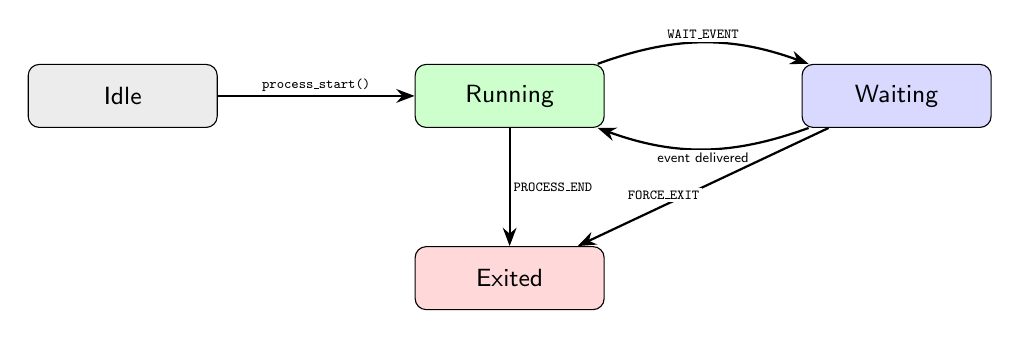
\begin{tikzpicture}[
    state/.style={draw, rounded corners, minimum width=2.4cm,
                  minimum height=0.8cm, font=\small\sffamily, fill=#1},
    every edge/.style={draw, ->, >=Stealth, thick},
    lbl/.style={font=\tiny\sffamily, fill=white, inner sep=1pt},
    node distance=1.8cm and 2.5cm
  ]

  \node[state=gray!15]   (idle)    {Idle};
  \node[state=green!20, right=of idle]  (running) {Running};
  \node[state=blue!15, right=of running] (waiting) {Waiting};
  \node[state=red!15, below=1.5cm of running]   (exited)  {Exited};

  \path (idle) edge node[lbl, above] {\texttt{process\_start()}} (running);
  \path (running) edge[bend left=20] node[lbl, above] {\texttt{WAIT\_EVENT}} (waiting);
  \path (waiting) edge[bend left=20] node[lbl, below] {event delivered} (running);
  \path (running) edge node[lbl, right] {\texttt{PROCESS\_END}} (exited);
  \path (waiting) edge node[lbl, below left] {\texttt{FORCE\_EXIT}} (exited);

\end{tikzpicture}
\end{center}

\vspace{0.3em}
\begin{columns}[T]
\begin{column}{0.48\textwidth}
\textbf{Start:}
\begin{itemize}
  \item \texttt{tiku\_process\_start()} adds to list
  \item Posts \texttt{TIKU\_EVENT\_INIT}
  \item Sets \texttt{is\_running = 1}
\end{itemize}
\end{column}
\begin{column}{0.48\textwidth}
\textbf{Exit:}
\begin{itemize}
  \item Automatic on \texttt{PROCESS\_END}
  \item Or \texttt{PROCESS\_EXIT()} (early)
  \item Or \texttt{FORCE\_EXIT} event (kill)
  \item Removed from linked list
\end{itemize}
\end{column}
\end{columns}
\end{frame}

% ---------------------------------------------------------------------------
\begin{frame}[fragile]{Key Process API}
\begin{table}
\centering
\small
\begin{tabular}{@{}lp{8cm}@{}}
\toprule
\textbf{Function / Macro} & \textbf{Description} \\
\midrule
\texttt{tiku\_process\_start(p, data)}  & Add process to list, post INIT event \\
\texttt{tiku\_process\_exit(p)}         & Remove process from list, mark inactive \\
\texttt{tiku\_process\_post(p, ev, d)}  & Post event to process (or broadcast if \texttt{p = NULL}) \\
\texttt{tiku\_process\_poll(p)}         & Post POLL event (safe from ISR) \\
\texttt{tiku\_process\_run()}           & Dequeue and dispatch one event \\
\midrule
\texttt{TIKU\_PROCESS\_BEGIN()}         & Start of protothread body \\
\texttt{TIKU\_PROCESS\_END()}           & End of protothread body \\
\texttt{TIKU\_PROCESS\_WAIT\_EVENT()}   & Yield until any event \\
\texttt{TIKU\_PROCESS\_WAIT\_EVENT\_UNTIL(c)} & Yield until condition \texttt{c} is true \\
\texttt{TIKU\_PROCESS\_YIELD()}         & Cooperative yield \\
\texttt{TIKU\_PROCESS\_EXIT()}          & Early exit from protothread \\
\texttt{TIKU\_THIS()}                   & Pointer to current process \\
\bottomrule
\end{tabular}
\end{table}
\end{frame}

% ===========================================================================
\section{Protothread Mechanics}
% ===========================================================================

\begin{frame}[fragile]{How Protothreads Work}
\begin{columns}[T]
\begin{column}{0.50\textwidth}
\textbf{What you write:}
\begin{lstlisting}[style=cstyle]
TIKU_PROCESS_THREAD(led, ev, data)
{
    TIKU_PROCESS_BEGIN();

    while (1) {
        TIKU_PROCESS_WAIT_EVENT_UNTIL(
            ev == TIKU_EVENT_TIMER);
        tiku_common_led1_toggle();
    }

    TIKU_PROCESS_END();
}
\end{lstlisting}
\end{column}

\begin{column}{0.46\textwidth}
\textbf{What the compiler sees:}
\begin{lstlisting}[style=cstyle, basicstyle=\ttfamily\tiny]
char thread_led(struct pt *pt,
    tiku_event_t ev, ...) {
  char PT_YIELD_FLAG = 1;
  switch (pt->lc) {
  case 0:  /* PROCESS_BEGIN */

    while (1) {
  case __LINE__:  /* WAIT_EVENT */
      if (!(ev == TIKU_EVENT_TIMER))
        return PT_YIELDED;
      toggle_led();
    }

  }  /* PROCESS_END */
  pt->lc = 0;
  return PT_ENDED;
}
\end{lstlisting}
\end{column}
\end{columns}

\vspace{0.3em}
\begin{alertblock}{Important Rule}
\textbf{No local variables across yield points.}
The switch/case jump skips initializers.
Use process-local storage or \texttt{static} variables instead.
\end{alertblock}
\end{frame}

% ---------------------------------------------------------------------------
\begin{frame}[fragile]{Protothread Return Codes}
\begin{table}
\centering
\begin{tabular}{@{}llp{7cm}@{}}
\toprule
\textbf{Code} & \textbf{Value} & \textbf{Meaning} \\
\midrule
\texttt{PT\_WAITING} & 0 & Blocked on a condition \\
\texttt{PT\_YIELDED} & 1 & Voluntarily yielded, ready to resume \\
\texttt{PT\_EXITED}  & 2 & Early exit (\texttt{PT\_EXIT}) \\
\texttt{PT\_ENDED}   & 3 & Reached \texttt{PT\_END} naturally \\
\bottomrule
\end{tabular}
\end{table}

\vspace{0.5em}
The scheduler uses these to manage process lifecycle:
\begin{itemize}
  \item \texttt{PT\_WAITING} or \texttt{PT\_YIELDED} --- process stays active
  \item \texttt{PT\_EXITED} or \texttt{PT\_ENDED} --- scheduler auto-calls \texttt{tiku\_process\_exit()}
  \item \texttt{PT\_SCHEDULE(f)} macro: true if thread still running
        (\texttt{f < PT\_EXITED})
\end{itemize}
\end{frame}

% ===========================================================================
\section{Events \& Communication}
% ===========================================================================

\begin{frame}[fragile]{Posting Events}
\begin{lstlisting}[style=cstyle, title={Post to a single process}]
#define EVENT_NEW_DATA (TIKU_EVENT_USER + 0)

/* Post with data payload (cast to void*) */
tiku_process_post(&consumer, EVENT_NEW_DATA, (void *)(intptr_t)value);
\end{lstlisting}

\begin{lstlisting}[style=cstyle, title={Broadcast to all processes}]
tiku_process_post(TIKU_PROCESS_BROADCAST, EVENT_HEARTBEAT, NULL);
/* TIKU_PROCESS_BROADCAST is NULL --- iterates entire process list */
\end{lstlisting}

\begin{lstlisting}[style=cstyle, title={Poll from ISR}]
/* Inside an interrupt handler */
tiku_process_poll(&sensor_process);
/* Posts TIKU_EVENT_POLL, wakes the process */
\end{lstlisting}

\vspace{0.3em}
\begin{block}{ISR Safety}
All post/poll functions use atomic sections ---
safe to call from interrupt context.
Queue holds 32 events; returns 0 if full.
\end{block}
\end{frame}

% ---------------------------------------------------------------------------
\begin{frame}[fragile]{Receiving Events}
\begin{lstlisting}[style=cstyle, title={Wait for any event}]
TIKU_PROCESS_WAIT_EVENT();
/* ev and data are set when process resumes */
\end{lstlisting}

\begin{lstlisting}[style=cstyle, title={Wait for a specific event}]
TIKU_PROCESS_WAIT_EVENT_UNTIL(ev == TIKU_EVENT_TIMER);
/* Ignores all other events, only wakes on TIMER */
\end{lstlisting}

\begin{lstlisting}[style=cstyle, title={Event dispatch loop pattern}]
while (1) {
    TIKU_PROCESS_WAIT_EVENT();

    if (ev == TIKU_EVENT_TIMER) {
        /* handle timer */
    } else if (ev == EVENT_NEW_DATA) {
        int value = (int)(intptr_t)data;
        /* handle data */
    } else if (ev == TIKU_EVENT_EXIT) {
        /* cleanup and exit */
        TIKU_PROCESS_EXIT();
    }
}
\end{lstlisting}
\end{frame}

% ===========================================================================
\section{Channels (Typed IPC)}
% ===========================================================================

\begin{frame}[fragile]{Channel: Type-Safe Message Passing}
\begin{lstlisting}[style=cstyle, title={Declare a channel}]
struct sensor_msg {
    uint16_t seq;
    uint16_t value;
};

/* Creates: sensor_ch, sensor_ch_init(), sensor_ch_put(), sensor_ch_get() */
TIKU_CHANNEL_DECLARE(sensor_ch, struct sensor_msg, 4);  /* depth = 4 */
\end{lstlisting}

\begin{columns}[T]
\begin{column}{0.48\textwidth}
\begin{lstlisting}[style=cstyle, title={Producer}]
struct sensor_msg msg;
msg.seq   = seq++;
msg.value = read_adc();

if (sensor_ch_put(&msg)) {
    /* notify consumer */
    tiku_process_post(&consumer,
        EVENT_DATA_READY, NULL);
}
\end{lstlisting}
\end{column}

\begin{column}{0.48\textwidth}
\begin{lstlisting}[style=cstyle, title={Consumer}]
TIKU_PROCESS_WAIT_EVENT_UNTIL(
    ev == EVENT_DATA_READY);

struct sensor_msg msg;
while (sensor_ch_get(&msg)) {
    /* process msg.seq, msg.value */
}
\end{lstlisting}
\end{column}
\end{columns}

\vspace{0.3em}
\begin{block}{Channel Internals}
Circular buffer, ISR-safe, compile-time type checking.
Decouples producer and consumer rates.
\end{block}
\end{frame}

% ---------------------------------------------------------------------------
\begin{frame}[fragile]{Channel Data Structure \& API}
\begin{columns}[T]
\begin{column}{0.48\textwidth}
\begin{lstlisting}[style=cstyle,
  title={kernel/process/tiku\_process.h}]
typedef struct tiku_channel {
    uint8_t *buf;
    uint8_t  msg_size;
    uint8_t  capacity;
    volatile uint8_t head;
    volatile uint8_t count;
} tiku_channel_t;
\end{lstlisting}

\begin{itemize}
  \item Caller-provided static buffer
  \item \texttt{volatile} head/count for ISR safety
  \item \texttt{memcpy}-based put/get
\end{itemize}
\end{column}

\begin{column}{0.48\textwidth}
\begin{table}
\centering
\small
\begin{tabular}{@{}lp{3.8cm}@{}}
\toprule
\textbf{Function} & \textbf{Description} \\
\midrule
\texttt{\_init()} & Wire buffer, set head/count=0 \\
\texttt{\_put(msg)} & Copy msg to tail; returns 1/0 \\
\texttt{\_get(out)} & Copy head to out; returns 1/0 \\
\texttt{is\_empty()} & True if count == 0 \\
\texttt{free()} & Remaining capacity \\
\bottomrule
\end{tabular}
\end{table}

\vspace{0.3em}
\texttt{TIKU\_CHANNEL\_DECLARE} generates
typed inline wrappers --- no raw pointer
casts needed at the call site.
\end{column}
\end{columns}
\end{frame}

% ===========================================================================
\section{Local Storage}
% ===========================================================================

\begin{frame}[fragile]{Process-Local Storage}

\begin{lstlisting}[style=cstyle, title={Declaring process with local storage}]
struct blink_state {
    uint16_t count;
    uint8_t  led_on;
};

TIKU_PROCESS_TYPED(blink_proc, "Blink", struct blink_state);
\end{lstlisting}

\begin{lstlisting}[style=cstyle, title={Using local storage inside protothread}]
TIKU_PROCESS_THREAD(blink_proc, ev, data)
{
    /* Get typed pointer ABOVE PROCESS_BEGIN (stack variable) */
    struct blink_state *s = blink_proc_local();

    TIKU_PROCESS_BEGIN();

    s->count = 0;
    s->led_on = 0;

    while (1) {
        TIKU_PROCESS_WAIT_EVENT_UNTIL(ev == TIKU_EVENT_TIMER);
        s->count++;
        s->led_on = !s->led_on;
    }

    TIKU_PROCESS_END();
}
\end{lstlisting}

\begin{alertblock}{Rule}
Assign the local pointer \textbf{above} \texttt{PROCESS\_BEGIN()}.
The pointer itself is a stack variable, but the storage it points to
persists across yields.
\end{alertblock}
\end{frame}

% ===========================================================================
\section{Scheduler}
% ===========================================================================

\begin{frame}[fragile]{Scheduler Loop}
\begin{columns}[T]
\begin{column}{0.50\textwidth}
\begin{lstlisting}[style=cstyle,
  title={kernel/scheduler/tiku\_sched.c}]
void tiku_sched_loop(void)
{
    /* Start autostart processes */
    tiku_autostart_start(
        tiku_autostart_processes);

    while (sched_state ==
           TIKU_SCHED_RUNNING) {

        /* 1. Drain all pending events */
        while (tiku_sched_run_once())
            ;

        /* 2. If truly idle, call hook */
        /* (enter low-power mode) */
        if (!tiku_sched_has_pending()
            && idle_hook) {
            idle_hook();
        }
    }
}
\end{lstlisting}
\end{column}

\begin{column}{0.46\textwidth}
\textbf{Execution flow:}
\begin{enumerate}
  \item Boot calls \texttt{tiku\_sched\_loop()}
  \item Autostart processes are started
  \item Loop: drain event queue
  \item Each \texttt{run\_once()} dequeues
        one event and dispatches it
  \item When idle, call hook (LPM)
  \item ISR posts event $\rightarrow$ CPU wakes
  \item Repeat
\end{enumerate}

\vspace{0.3em}
\begin{block}{Idle Hook}
\begin{lstlisting}[style=cstyle, basicstyle=\ttfamily\tiny]
tiku_sched_set_idle_hook(
    enter_lpm3);
/* Called when no events pending */
\end{lstlisting}
\end{block}
\end{column}
\end{columns}
\end{frame}

% ---------------------------------------------------------------------------
\begin{frame}[fragile]{Autostart}
\begin{lstlisting}[style=cstyle, title={Register processes for autostart}]
/* Single process */
TIKU_AUTOSTART_PROCESSES(&blink_process);

/* Multiple processes */
TIKU_AUTOSTART_PROCESSES(&producer, &consumer, &logger);
\end{lstlisting}

\vspace{0.3em}
\begin{itemize}
  \item Creates a NULL-terminated array of process pointers
  \item Scheduler iterates and calls \texttt{tiku\_process\_start()} on each
  \item Every process receives \texttt{TIKU\_EVENT\_INIT} as its first event
  \item Processes are started in declaration order
\end{itemize}

\vspace{0.3em}
\begin{block}{Manual Start (without autostart)}
\begin{lstlisting}[style=cstyle]
/* Start a process at runtime */
tiku_process_start(&my_process, NULL);

/* Start via scheduler wrapper */
tiku_sched_start(&my_process, NULL);
\end{lstlisting}
\end{block}
\end{frame}

% ===========================================================================
\section{Examples}
% ===========================================================================

\begin{frame}[fragile]{Example 1: LED Blink}
\begin{lstlisting}[style=cstyle, title={examples/01\_blink/blink.c}]
static struct tiku_timer blink_timer;

TIKU_PROCESS(blink_process, "Blink");

TIKU_PROCESS_THREAD(blink_process, ev, data)
{
    TIKU_PROCESS_BEGIN();

    tiku_common_led1_init();
    tiku_timer_set_event(&blink_timer, TIKU_CLOCK_SECOND);

    while (1) {
        TIKU_PROCESS_WAIT_EVENT_UNTIL(ev == TIKU_EVENT_TIMER);
        tiku_common_led1_toggle();
        tiku_timer_reset(&blink_timer);   /* drift-free restart */
    }

    TIKU_PROCESS_END();
}

TIKU_AUTOSTART_PROCESSES(&blink_process);
\end{lstlisting}
\end{frame}

% ---------------------------------------------------------------------------
\begin{frame}[fragile]{Example 2: Dual Blink (Two Processes)}
\begin{lstlisting}[style=cstyle, title={examples/02\_dual\_blink/dual\_blink.c}]
static struct tiku_timer red_timer, green_timer;

TIKU_PROCESS(red_blink,   "Red Blink");      /* 500 ms */
TIKU_PROCESS(green_blink, "Green Blink");     /* 1.5 s  */

TIKU_PROCESS_THREAD(red_blink, ev, data) {
    TIKU_PROCESS_BEGIN();
    tiku_common_led1_init();
    tiku_timer_set_event(&red_timer, TIKU_CLOCK_SECOND / 2);
    while (1) {
        TIKU_PROCESS_WAIT_EVENT_UNTIL(ev == TIKU_EVENT_TIMER);
        tiku_common_led1_toggle();
        tiku_timer_reset(&red_timer);
    }
    TIKU_PROCESS_END();
}

TIKU_PROCESS_THREAD(green_blink, ev, data) {
    TIKU_PROCESS_BEGIN();
    tiku_common_led2_init();
    tiku_timer_set_event(&green_timer, (3 * TIKU_CLOCK_SECOND) / 2);
    while (1) {
        TIKU_PROCESS_WAIT_EVENT_UNTIL(ev == TIKU_EVENT_TIMER);
        tiku_common_led2_toggle();
        tiku_timer_reset(&green_timer);
    }
    TIKU_PROCESS_END();
}

TIKU_AUTOSTART_PROCESSES(&red_blink, &green_blink);
\end{lstlisting}
\end{frame}

% ---------------------------------------------------------------------------
\begin{frame}[fragile]{Example 3: Producer--Consumer}
\begin{lstlisting}[style=cstyle, title={examples/04\_multi\_process/multi\_process.c (simplified)}]
#define EVENT_NEW_DATA (TIKU_EVENT_USER + 0)

TIKU_PROCESS(producer, "Producer");
TIKU_PROCESS(consumer, "Consumer");

TIKU_PROCESS_THREAD(producer, ev, data) {
    static uint16_t counter = 0;
    TIKU_PROCESS_BEGIN();
    tiku_timer_set_event(&prod_timer, TIKU_CLOCK_SECOND);
    while (1) {
        TIKU_PROCESS_WAIT_EVENT_UNTIL(ev == TIKU_EVENT_TIMER);
        tiku_process_post(&consumer, EVENT_NEW_DATA,
                          (void *)(intptr_t)counter++);
        tiku_timer_reset(&prod_timer);
    }
    TIKU_PROCESS_END();
}

TIKU_PROCESS_THREAD(consumer, ev, data) {
    TIKU_PROCESS_BEGIN();
    while (1) {
        TIKU_PROCESS_WAIT_EVENT_UNTIL(ev == EVENT_NEW_DATA);
        int value = (int)(intptr_t)data;
        /* process value */
    }
    TIKU_PROCESS_END();
}
TIKU_AUTOSTART_PROCESSES(&producer, &consumer);
\end{lstlisting}
\end{frame}

% ---------------------------------------------------------------------------
\begin{frame}[fragile]{Example 4: Broadcast}
\begin{lstlisting}[style=cstyle, title={examples/07\_broadcast/broadcast.c (simplified)}]
#define EVENT_HEARTBEAT (TIKU_EVENT_USER + 0)

TIKU_PROCESS(controller, "Controller");
TIKU_PROCESS(listener_a, "Listener A");
TIKU_PROCESS(listener_b, "Listener B");

TIKU_PROCESS_THREAD(controller, ev, data) {
    TIKU_PROCESS_BEGIN();
    tiku_timer_set_event(&hb_timer, TIKU_CLOCK_SECOND);
    while (1) {
        TIKU_PROCESS_WAIT_EVENT_UNTIL(ev == TIKU_EVENT_TIMER);
        tiku_process_post(TIKU_PROCESS_BROADCAST, EVENT_HEARTBEAT, NULL);
        tiku_timer_reset(&hb_timer);
    }
    TIKU_PROCESS_END();
}

TIKU_PROCESS_THREAD(listener_a, ev, data) {
    TIKU_PROCESS_BEGIN();
    while (1) {
        TIKU_PROCESS_WAIT_EVENT_UNTIL(ev == EVENT_HEARTBEAT);
        tiku_common_led1_toggle();
    }
    TIKU_PROCESS_END();
}
TIKU_AUTOSTART_PROCESSES(&controller, &listener_a, &listener_b);
\end{lstlisting}
\end{frame}

% ---------------------------------------------------------------------------
\begin{frame}[fragile]{Example 5: Channel IPC}
\begin{lstlisting}[style=cstyle, title={examples/09\_channel/channel.c (simplified)}]
struct sensor_msg { uint16_t seq; uint16_t value; };
TIKU_CHANNEL_DECLARE(sensor_ch, struct sensor_msg, 4);
#define EVENT_DATA_READY (TIKU_EVENT_USER + 0)

TIKU_PROCESS_THREAD(sensor_proc, ev, data) {
    static uint16_t seq = 0;
    TIKU_PROCESS_BEGIN();
    sensor_ch_init();
    tiku_timer_set_event(&sensor_timer, TIKU_CLOCK_SECOND / 2);
    while (1) {
        TIKU_PROCESS_WAIT_EVENT_UNTIL(ev == TIKU_EVENT_TIMER);
        struct sensor_msg msg = { seq++, seq * 10 };
        if (sensor_ch_put(&msg))
            tiku_process_post(&display_proc, EVENT_DATA_READY, NULL);
        tiku_timer_reset(&sensor_timer);
    }
    TIKU_PROCESS_END();
}

TIKU_PROCESS_THREAD(display_proc, ev, data) {
    TIKU_PROCESS_BEGIN();
    while (1) {
        TIKU_PROCESS_WAIT_EVENT_UNTIL(ev == EVENT_DATA_READY);
        struct sensor_msg msg;
        while (sensor_ch_get(&msg)) { /* drain all */ }
    }
    TIKU_PROCESS_END();
}
\end{lstlisting}
\end{frame}

% ===========================================================================
\section{Test Suite}
% ===========================================================================

\begin{frame}[fragile]{Test Configuration}
\begin{columns}[T]
\begin{column}{0.48\textwidth}
\begin{lstlisting}[style=cstyle, title={tests/tiku\_test\_config.h}]
#define TEST_ENABLE 1

/* Process test flags */
#define TEST_PROCESS_LIFECYCLE     1
#define TEST_PROCESS_EVENTS        1
#define TEST_PROCESS_YIELD         1
#define TEST_PROCESS_BROADCAST     1
#define TEST_PROCESS_POLL          1
#define TEST_PROCESS_QUEUE         1
#define TEST_PROCESS_LOCAL         1
#define TEST_PROCESS_BROADCAST_EXIT 1
#define TEST_PROCESS_GRACEFUL_EXIT  1
#define TEST_PROCESS_CURRENT_CLEARED 1
\end{lstlisting}
\end{column}

\begin{column}{0.48\textwidth}
\textbf{Run on target:}
\begin{lstlisting}[style=cstyle, basicstyle=\ttfamily\tiny]
# Enable flags, then:
make flash MCU=msp430fr5969
make monitor
\end{lstlisting}

\vspace{0.5em}
\textbf{10 test cases covering:}
\begin{itemize}
  \item Process start/exit lifecycle
  \item Event posting and reception
  \item Cooperative yielding phases
  \item Broadcast to multiple processes
  \item Poll from ISR context
  \item Queue capacity and overflow
  \item Local storage persistence
  \item Broadcast exit safety
  \item Graceful vs force exit
  \item Current process clearing
\end{itemize}
\end{column}
\end{columns}
\end{frame}

% ---------------------------------------------------------------------------
\begin{frame}{Test Cases Overview}
\begin{table}
\centering
\small
\begin{tabular}{@{}clp{6.5cm}@{}}
\toprule
\textbf{\#} & \textbf{Test Flag} & \textbf{What It Verifies} \\
\midrule
1  & \texttt{LIFECYCLE}       & start posts INIT; END auto-exits \\
2  & \texttt{EVENTS}          & custom event posting and reception \\
3  & \texttt{YIELD}           & multi-phase yield with continuation \\
4  & \texttt{BROADCAST}       & single post reaches all processes \\
5  & \texttt{POLL}            & \texttt{tiku\_process\_poll()} delivers POLL event \\
6  & \texttt{QUEUE}           & empty/full/length/space; overflow returns 0 \\
7  & \texttt{LOCAL}           & WITH\_LOCAL and TYPED storage persists across yields \\
8  & \texttt{BROADCAST\_EXIT} & process exiting mid-broadcast doesn't corrupt list \\
9  & \texttt{GRACEFUL\_EXIT}  & EXIT event: process can do cleanup; FORCE\_EXIT kills \\
10 & \texttt{CURRENT\_CLEARED} & \texttt{TIKU\_THIS()} is NULL outside dispatch \\
\bottomrule
\end{tabular}
\end{table}
\end{frame}

% ===========================================================================
\section{Common Patterns}
% ===========================================================================

\begin{frame}[fragile]{Pattern Reference}
\begin{columns}[T]
\begin{column}{0.48\textwidth}
\begin{lstlisting}[style=cstyle, title={Periodic timer}]
static struct tiku_timer t;
/* in PROCESS_THREAD: */
tiku_timer_set_event(&t,
    TIKU_CLOCK_SECOND);
while (1) {
    TIKU_PROCESS_WAIT_EVENT_UNTIL(
        ev == TIKU_EVENT_TIMER);
    /* do work */
    tiku_timer_reset(&t);
}
\end{lstlisting}

\begin{lstlisting}[style=cstyle, title={Graceful shutdown}]
while (1) {
    TIKU_PROCESS_WAIT_EVENT();
    if (ev == TIKU_EVENT_EXIT) {
        /* cleanup */
        TIKU_PROCESS_EXIT();
    }
    /* normal work */
}
\end{lstlisting}
\end{column}

\begin{column}{0.48\textwidth}
\begin{lstlisting}[style=cstyle, title={ISR to process}]
/* In ISR: */
tiku_process_poll(&my_proc);

/* In process: */
TIKU_PROCESS_WAIT_EVENT_UNTIL(
    ev == TIKU_EVENT_POLL);
/* handle hardware event */
\end{lstlisting}

\begin{lstlisting}[style=cstyle, title={Multi-event dispatch}]
while (1) {
    TIKU_PROCESS_WAIT_EVENT();
    switch (ev) {
    case TIKU_EVENT_TIMER:
        handle_timer(); break;
    case EVENT_BTN:
        handle_button(); break;
    case TIKU_EVENT_EXIT:
        TIKU_PROCESS_EXIT();
    }
}
\end{lstlisting}
\end{column}
\end{columns}
\end{frame}

% ===========================================================================
\section{Summary}
% ===========================================================================

\begin{frame}{Summary}
\begin{columns}[T]
\begin{column}{0.48\textwidth}
\begin{block}{Process Model}
\begin{itemize}
  \item Stackless protothreads (2 bytes each)
  \item Event-driven cooperative scheduling
  \item 32-entry circular event queue
  \item ISR-safe posting and polling
  \item Autostart mechanism
  \item Broadcast events
  \item Per-process local storage
\end{itemize}
\end{block}
\end{column}

\begin{column}{0.48\textwidth}
\begin{block}{Communication}
\begin{itemize}
  \item Direct events: one-to-one
  \item Broadcast: one-to-all
  \item Channels: typed message queues
  \item Poll: ISR to process notification
\end{itemize}
\end{block}

\vspace{0.3em}
\begin{block}{Testing}
10 test cases covering lifecycle, events, yield,
broadcast, poll, queue, local storage, exit safety.
\end{block}
\end{column}
\end{columns}
\end{frame}

% ---------------------------------------------------------------------------
\begin{frame}{Thank You}
\begin{center}
\Large\textbf{TikuOS Processes}\\[0.5em]
\normalsize Protothreads \& Events for Physical AI Endpoints\\[1.5em]

\begin{tabular}{rl}
  Repository: & \url{https://github.com/tikuos/tikuOS} \\
  License:    & Apache 2.0 \\
  API Header: & \texttt{kernel/process/tiku\_process.h} \\
  Examples:   & \texttt{examples/01\_blink/} \ldots\ \texttt{examples/09\_channel/} \\
  Tests:      & \texttt{tests/test\_process.c} \\
\end{tabular}
\end{center}
\end{frame}

\end{document}
